\documentclass[conference]{IEEEtran}
\IEEEoverridecommandlockouts
% The preceding line is only needed to identify funding in the first footnote. If that is unneeded, please comment it out.
\usepackage{cite}
\usepackage{amsmath,amssymb,amsfonts}
\usepackage{algorithmic}
\usepackage{graphicx}
\usepackage{textcomp}
\usepackage{xcolor}
\def\BibTeX{{\rm B\kern-.05em{\sc i\kern-.025em b}\kern-.08em
    T\kern-.1667em\lower.7ex\hbox{E}\kern-.125emX}}
\begin{document}

\title{Pengembangan \textit{Firmware Tracker} Bus Kampus dengan Modul GNSS pada Platform STM32}

\author{\IEEEauthorblockN{Airlangga Rasyad Fidiyanto, I Wayan Mustika, Agus Bejo}
\IEEEauthorblockA{
Departemen Teknik Elektro dan Teknologi Informasi\\
Fakultas Teknik, Universitas Gadjah Mada\\
Yogyakarta, Indonesia \\
fairlanggarasyad@mail.ugm.ac.id \{wmustika, agusbj\}@ugm.ac.id}
}

\maketitle

\begin{abstract}
Penelitian ini bertujuan untuk mengevaluasi performa dari modul GNSS Teseo-LIV3FL dan mengembangkan firmware pelacak Bus Trans Gadjah Mada menggunakan platform STM32. Evaluasi performa \textit{multi-constellation} modul dilakukan dengan mengatur modul untuk menerima isyarat dari berbagai konstelasi GNSS. Selain itu, firmware yang dikembangkan memiliki fitur geofencing untuk menentukan apakah posisi bus saat ini berada di dalam lingkungan kampus Universitas Gadjah Mada atau tidak. \textit{Firmware} ini akan diujikan pada Rute 1B Trans Gadjah Mada.
\end{abstract}

\begin{IEEEkeywords}
STM32, Teseo-LIV3FL, pengembangan firmware, pelacakan posisi, algoritma daya rendah, multi-cosntellation
\end{IEEEkeywords}

\section{Pendahuluan}
Bus adalah salah satu moda transportasi dalam kota yang paling populer di Indonesia. Daerah Istimewa Yogyakarta telah menyediakan dua layanan bus publik, yaitu Trans Jogja dan Teman Bus. Salah satu faktor yang membuat penggunaan bus cukup populer adalah cakupan wilayahnya yang luas dan biayanya yang terjangkau \cite{Rohani2013}. Selain itu, lalu lintas yang padat dan lahan parkir yang terbatas juga menjadi motivasi beberapa orang untuk menggunakan transportasi publik. Jika peningkatan jumlah penduduk pada suatu daerah sangat tinggi, maka dibutuhkan fasilitas transportasi umum yang layak seperti bus \cite{Sutandi2015}.

Pada awal bulan Maret 2022, Rektor Universitas Gadjah Mada, Prof. Ir. Panut Mulyono, M.Eng., D.Eng., meluncurkan dua buah bus listrik untuk transportasi internal kampus. Kedua bus ini merupakan inovasi dari UGM untuk memudahkan mobilisasi mahasiswa di area kampus seluas 183,36 hektar dengan mengurangi penggunaan energi fosil secara bersamaan. Setiap bus akan memutari UGM sebanyak sepuluh kali dengan setiap putaran membutuhkan satu jam. Dengan adanya fasilitas bus kampus Trans Gadjah Mada diharapkan dapat membuat lingkungan kampus menjadi lebih nyaman dan kondusif.

Saat ini, civitas akademika Universitas Gadjah Mada hanya dapat bergantung terhadap rute yang telah dipublikasikan oleh Direktorat Pengelolaan dan Pemeliharaan Aset Universitas Gadjah Mada. Padahal, kondisi di lapangan menunjukan bahwa waktu kedatangan Bus Trans Gadjah Mada tidak selalu tepat waktu. Sebagai contoh, jika lalu lintas lancar maka waktu kedatangan Bus bisa lebih cepat hingga 5 menit dari waktu pada jadwal. 

Masalah serupa juga terjadi di India. Berdasarkan penelitian \cite{Sutar2016}, masyarakat India hanya mengetahui waktu kedatangan bus berdasarkan jadwal saja tanpa mengetahui posisi terbaru dari bus yang akan ditumpangi. Penelitian yang dilakukan oleh \cite{Sneha2014} menunjukkan bahwa sistem pelacak berbasis GNSS telah diimplementasikan di beberapa negara, tetapi belum diimplementasikan di Indonesia, khususnya di lingkungan Universitas Gadjah Mada.

Untuk mengatasi masalah ketidakpastian waktu kedatangan Bus Trans Gadjah Mada, dibutuhkan sistem pelacakan yang akurat dan terpercaya. Salah satu teknologi sistem navigasi berbasis satelit yang dapat menunjukkan posisi secara akurat adalah Global Navigation Satellite System (GNSS). Dengan dikembangkannya firmware sistem pelacak lokasi bus Trans Gadjah Mada berbasis GNSS, diharapkan dapat membantu untuk melacak posisi bus secara akurat dan meningkatkan kepuasan pengguna.

\section{Penelitian Terkait}
Penelitian sebelumnya telah mengembangkan berbagai sistem pelacak kendaraan dengan berbagai macam pendekatan pada perangkat keras maupun perangkat lunak untuk berbagai aplikasi. Sebagai contoh, \cite{Ekhsan2022} merancang suatu sistem untuk melacak dompet dengan menggunakan TK-102 GPS Tracker.

Tim peneliti dari \textit{Vidyalankar Institute of Technology} telah merancang suatu sistem yang dapat mendeteksi lokasi dari kendaraan dan juga emisi CO yang dihasilkan. Pada sistem yang dirancang, digunakan \textit{development board} Arduino Uno yang berbasis mikrokontroler ATmega328. Ketika kandungan gas CO sudah melebihi ambang batas, sistem akan memutus pengiriman bahan bakar dan kemudian mengirimkan data koordinat dari modul GPS ke \textit{server} Apache yang telah dirancang \cite{Asha2022}.

Sebuah sistem \textit{speedometer} telah dirancang oleh \cite{Najmurrokhman2021}. Sistem tersebut menggunakan modul GPS untuk menghitung kecepatan dan koordinat lokasi kendaraan. Data kecepatan kendaraan didapat dari menghitung waktu yang dibutuhkan oleh kendaraan untuk berpindah dari satu titik ke titik lainnya. Data yang didapat dikirimkan dengan API Adafruit IO menggunakan modul SIM808.

Penelitian yang dilakukan oleh \cite{Mukhtar2015} dari \textit{University of London} menggunakan mikrokontroler AT89S52 dari keluarga 8051. Digunakan modul GPS M-89 yang diatur untuk menerima isyarat transmisi satelit pada frekuensi 1575.42 MHz. Data yang diterima akan ditampilkan pada layar LCD dan dikirimkan dengan modul GSM. Kemudian, data yang telah diterima akan ditampilkan pada situs web.

Sistem yang dirancang pada penelitian \cite{Widya2016} menggunakan modul GPS u-Blox Neo 6m. Penelitian ini memiliki kesamaan, yaitu objek yang akan dilacak adalah kendaraan bus. Sama seperti penelitian-penelitian sebelumnya, pada penelitian ini hanya digunakan satu buah konstelasi GNSS, yaitu GPS.

Namun, pada penelitian-penelitian di atas hanya digunakan satu buah konstelasi GNSS, yaitu GPS. Oleh karena itu, pada penelitian ini akan dirancang sistem pelacak kendaraan berbasis GNSS \textit{multi-constellation} dengan menggunakan modul GNSS Teseo-LIV3FL dan mikrokontroler STM32 WL55JC. Selain itu, sistem \textit{geofencing} yang telah ada dapat dikembangkan lebih lanjut seperti dapat mendeteksi apakah kendaraan sedang berhenti di halte atau tidak. Dengan begitu, penelitian ini diharapkan dapat memberikan kontribusi yang signifikan pada pengembangan sistem pelacak kendaraan berbasis GNSS.

\section{Metode Penelitian}
Penelitian ini dilakukan pada tahun 2023 menggunakan modul GNSS Teseo-LIV3FL dan \textit{development board} STM32 Nucleo-WL55JC1. Lokasi penelitian berada di lingkungan Universitas Gadjah Mada dan sekitarnya. Adapun konfigurasi konstelasi yang digunakan adalah GPS, BeiDou, Galileo, dan QZSS. Pada penelitian ini akan dilakukan empat pengujian. Pengujian \textit{rapid static survey} dan mode daya rendah hanya meninjau modul GNSS-nya saja, sedangkan dua pengujian lainnya akan menguji sistem secara keseluruhan.

\textit{Rapid Static Survey} dilakukan untuk meninjau performa modul GNSS dalam keadaan diam. Pengujian dilakukan dengan meletakan modul di satu tempat dan merekam data selama satu jam. Untuk menerima kalimat NMEA dari modul, digunakan perangkat USB \textit{to} TTL dengan konfigurasi \textit{baud rate} 9600 bps. Pengujian ini dilakukan dalam empat buah skenario, yaitu \textit{basement}, dalam ruangan, ruang semi terbuka, dan ruang terbuka. Lokasi setiap skenario \textit{Rapid Static Survey} ditunjukan oleh Tabel \ref{tab: 3-rss-location}.

\begin{table}[hbt!]
	\caption{Lokasi Pengujian \textit{Rapid Static Survey}}
	\centering
	\renewcommand{\arraystretch}{1.5}
	\begin{tabular}{cc}
		\hline
		\textbf{Skenario} & \textbf{Lokasi} \\\hline
		\textit{Basement} &Ruang Bawah Tanah Fisipol UGM\\
		Dalam Ruangan & Lantai 5 SGLC Fakultas Teknik UGM\\
		Ruangan Semi Terbuka &  Selasar Grha Sabha Pramana\\
		Ruang Terbuka & Lapangan Pancasila\\
		\hline
	\end{tabular}
	\label{tab: 3-rss-location}
\end{table}

Salah satu fitur unggulan dari modul GNSS Teseo-LIV3FL adalah memiliki mode daya rendah. Pengujian mode daya rendah akan meninjau arus yang mengalir pada modul ketika mode daya rendah diaktifkan. Algoritma mode daya rendah yang digunakan adalah algoritma periodik.

Fitur \textit{geofencing} berfungsi untuk memantau posisi dari suatu aset dalam wilayah tertentu. Salah satu impelementasi \textit{geofencing} adalah untuk menentukan jika posisi dari bus saat ini berada di dalam lingkungan Universitas Gadjah Mada atau tidak. Wilayah \textit{geofencing} didefinisikan sebagai lingkaran dengan radius 1 kilometer dengan pusat di koordinat (-7,771376; 110,377493). Pengujian dilakukan pada delapan belas titik acak di sekitar Universitas Gadjah Mada. \textit{Firmware} akan mengembalikan nilai satu jika posisi saat ini berada di dalam wilayah \textit{geofencing} dan nol untuk sebaliknya.

Selain untuk \textit{geofencing} di wilayah Universitas Gadjah Mada, fitur \textit{geofencing} juga dapat dikembangkan lebih lanjut untuk mendeteksi jika bus sedang berhenti di halte. Daerah \textit{geofence} setiap halte adalah lingkaran dengan jari-jari 10 meter dengan pusat lingkaran berada di koordinat halte. Pengujian \textit{geofencing} halte dilakukan di tujuh halte yang disinggahi oleh Bus Trans Gadjah Mada. Tabel \ref{tab: 3-geof-halte} menunjukan koordinat dari halte pada pengujian \textit{geofencing} halte.

\begin{table}[hbt!]
	\caption{Koordinat Halte Pengujian \textit{Geofencing} Halte}
	\centering
	\renewcommand{\arraystretch}{1.5}
	\begin{tabular}{cc}
		\hline
		\textbf{Halte} & \textbf{Koordinat} \\\hline
		6 & -7,769693; 110,373557 \\
		8 &-7,766077; 110,374062\\ 
		11 &-7,766508; 110,3706700\\
		13 & -7,766407; 110,3740824\\
		17 &-7,769712; 110,385479\\ 
		20 & -7,771089; 110,381336\\
		21 & -7,772668; 110,379638\\
		\hline
	\end{tabular}
	\label{tab: 3-geof-halte}
\end{table}

Setelah meninjau performa \textit{multi-constellation} pada modul GNSS dan \textit{geofence}, langkah selanjutnya adalah menguji sisetm secara keseluruhan di Bus Trans Gadjah Mada. Pada penelitian ini, rute yang dipilih adalah Rute 1B (Gambar \ref{fig: tgm-1b}). Waktu tempuh pengujian ini kurang lebih adalah selama satu jam yang diawali pada halte ke-14 dan diakhiri pada halte yang sama.

\begin{figure}[hbt!]
	\centering
	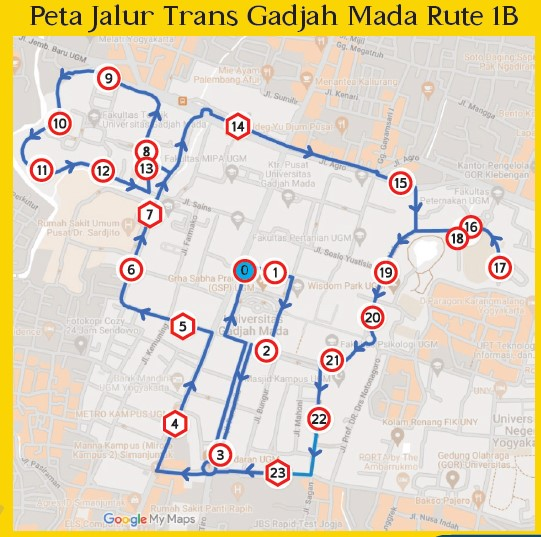
\includegraphics[width=6cm]{Peta-Jalur-Rute-1B.jpg}
	\caption{Rute 1B Trans Gadjah Mada}
	\label{fig: tgm-1b}
\end{figure}

\section{Hasil Pengujian}
\subsection{\textit{Rapid Static Survey}}
\begin{table*}[tbp]
	\centering
	\renewcommand{\arraystretch}{1.5}
	\caption{Rata-Rata Hasil Pengamatan \textit{Rapid Static Survey}}
	\label{tab: 4-rss-summary}
	\begin{tabular}{ccccccc}
		\hline
		\textbf{Skenario} & \textbf{HDOP} & \textbf{VDOP} & \textbf{PDOP} & \textbf{Visibilitas Satelit} & \textbf{CEP} & \textbf{MAD} \\
		&  & &  & (buah) & (m) & (m) \\
		\hline
		1 & 6,67 & 8,27 & 10,67 & 7,60 & 32,69 & 24,11 \\
		2 & 2,79 & 2,48 & 8,40 & 10,93 & 12,14 & 8,46 \\
		3 & 0,91 & 1,49 & 1,75 & 14,32 & 13,83 & 3,06 \\
		4 & 0,65 & 1,12 & 1,30 & 21,14 & 6,12 & 1,21 \\
		\hline
	\end{tabular}
\end{table*}

Pengujian \textit{rapid static survey} dilakukan dengan cara menaruh modul GNSS di satu titik selama 15 menit s.d. 2 jam. Setiap skenario pengujian dibedakan berdasarkan penghalang di sekitarnya. Pada penelitian ini, durasi dari pengujian di setiap skenario adalah selama 1 jam. Parameter yang diamati dalam pengujian ini adalah HDOP, VDOP, PDOP, visibilitas satelit, \textit{Circular Error Probability} (CEP), dan \textit{Mean Average Deviation} (MAD). Hasil pengujian setiap skenario ditunjukan oleh Tabel \ref{tab: 4-rss-summary}.

Skenario 1 dilakukan di \textit{basement} milik Fakultas Ilmu Sosial dan Politik UGM. Keadaan sekitar pengujian ditutupi oleh konstruksi beton dengan sedikit daerah terbuka yang memungkinkan sinar matahari untuk masuk. Keadaan tersebut tentunya akan sulit untuk ditembus oleh isyarat GNSS. Meskipun terhalang dengan beton, tetapi modul GNSS Teseo-LIV3FL dapat menerima isyarat GNSS dengan cukup baik ditunjukan oleh visibilitas satelit rata-rata sebanyak 7,60 buah. Berdasarkan Tabel X pada bagian sebelumnya menunjukan bahwa dengan nilai DOP yang didapat, hasil pengukuran posisi yang didapat sudah layak untuk digunakan. Selain itu, ketelitian hasil pengukuran modul Teseo-LIV3FL menurut nilai MAD dan CEP adalah sebesar 24,11 meter dan 32,69 meter.

Selanjutnya, Skenario 2 dilakukan di Lantai 5 SGLC Fakultas Teknik. Pemilihan lokasi tersebut ditujukan untuk menguji modul Teseo-LIV3FL di lingkungan yang sedikit lebih terbuka. Hasil pengujian menunjukan terjadi peningkatan performa pada modul Teseo-LIV3FL. Dapat dilihat bahwa rata-rata visibilitas satelit meningkat menjadi 10,92. Selain itu, rata-rata nilai HDOP dan VDOP sudah berada dalam standar minimum sedangkan PDOP-nya masih berada dalam kategori cukup. Tingkat kepresisian modul juga mengalami peningkatan seperti ditunjukan dengan nilai rata-rata CEP sebesar 12,13 meter dan MAD sebesar 8,46 meter.

Skenario 3 dilakukan di selasar Grha Sabha Pramana Universitas Gadjah Mada. Pengujian skenario ini dilakukan untuk meninjau performa modul GNSS di ruang semi-terbuka. Pada skenario ini, performa modul Teseo-LIV3FL menjadi lebih baik yang ditunjukan oleh penurunan nilai ketiga DOP. Nilai HDOP sudah termasuk dalam klasifikasi ideal, sedangkan VDOP dan HDOP berada dalam klasifikasi sangat baik. Selain itu, rata-rata visibilitas satelit meningkat menjadi 14,32. Pada pengujian ini terjadi sedikit peningkatan pada nilai CEP menjadi 13,83 meter, tetapi nilai MAD-nya menurun menjadi 6,12 meter.

 Terakhir, Skenario 4 dilakukan di Lapangan Pancasila Universitas Gadjah Mada. Lapangan pancasila dipilih karena merepresentasikan kondisi ideal penempatan modul GNSS, yaitu ruang terbuka tanpa halangan. Hasil pengujian skenario ini merupakan hasil paling baik dari tiga skenario sebelumnya dengan rata-rata visibilitas satelit 21,14. Nilai HDOP, VDOP, dan PDOP masih dalam rentang yang sama, tetapi sedikit lebih baik. Rata-rata nilai CEP dari pengujian ini adalah 6,12 meter  dan nilai MAD sebesar 1,21 meter. Meskipun nilai CEP yang didapat tidak sama dengan \textit{datasheet}, tetapi nilai tersebut sudah cukup baik untuk aplikasi pelacak kendaraan.

\begin{figure}[hbt!]
	\centering
	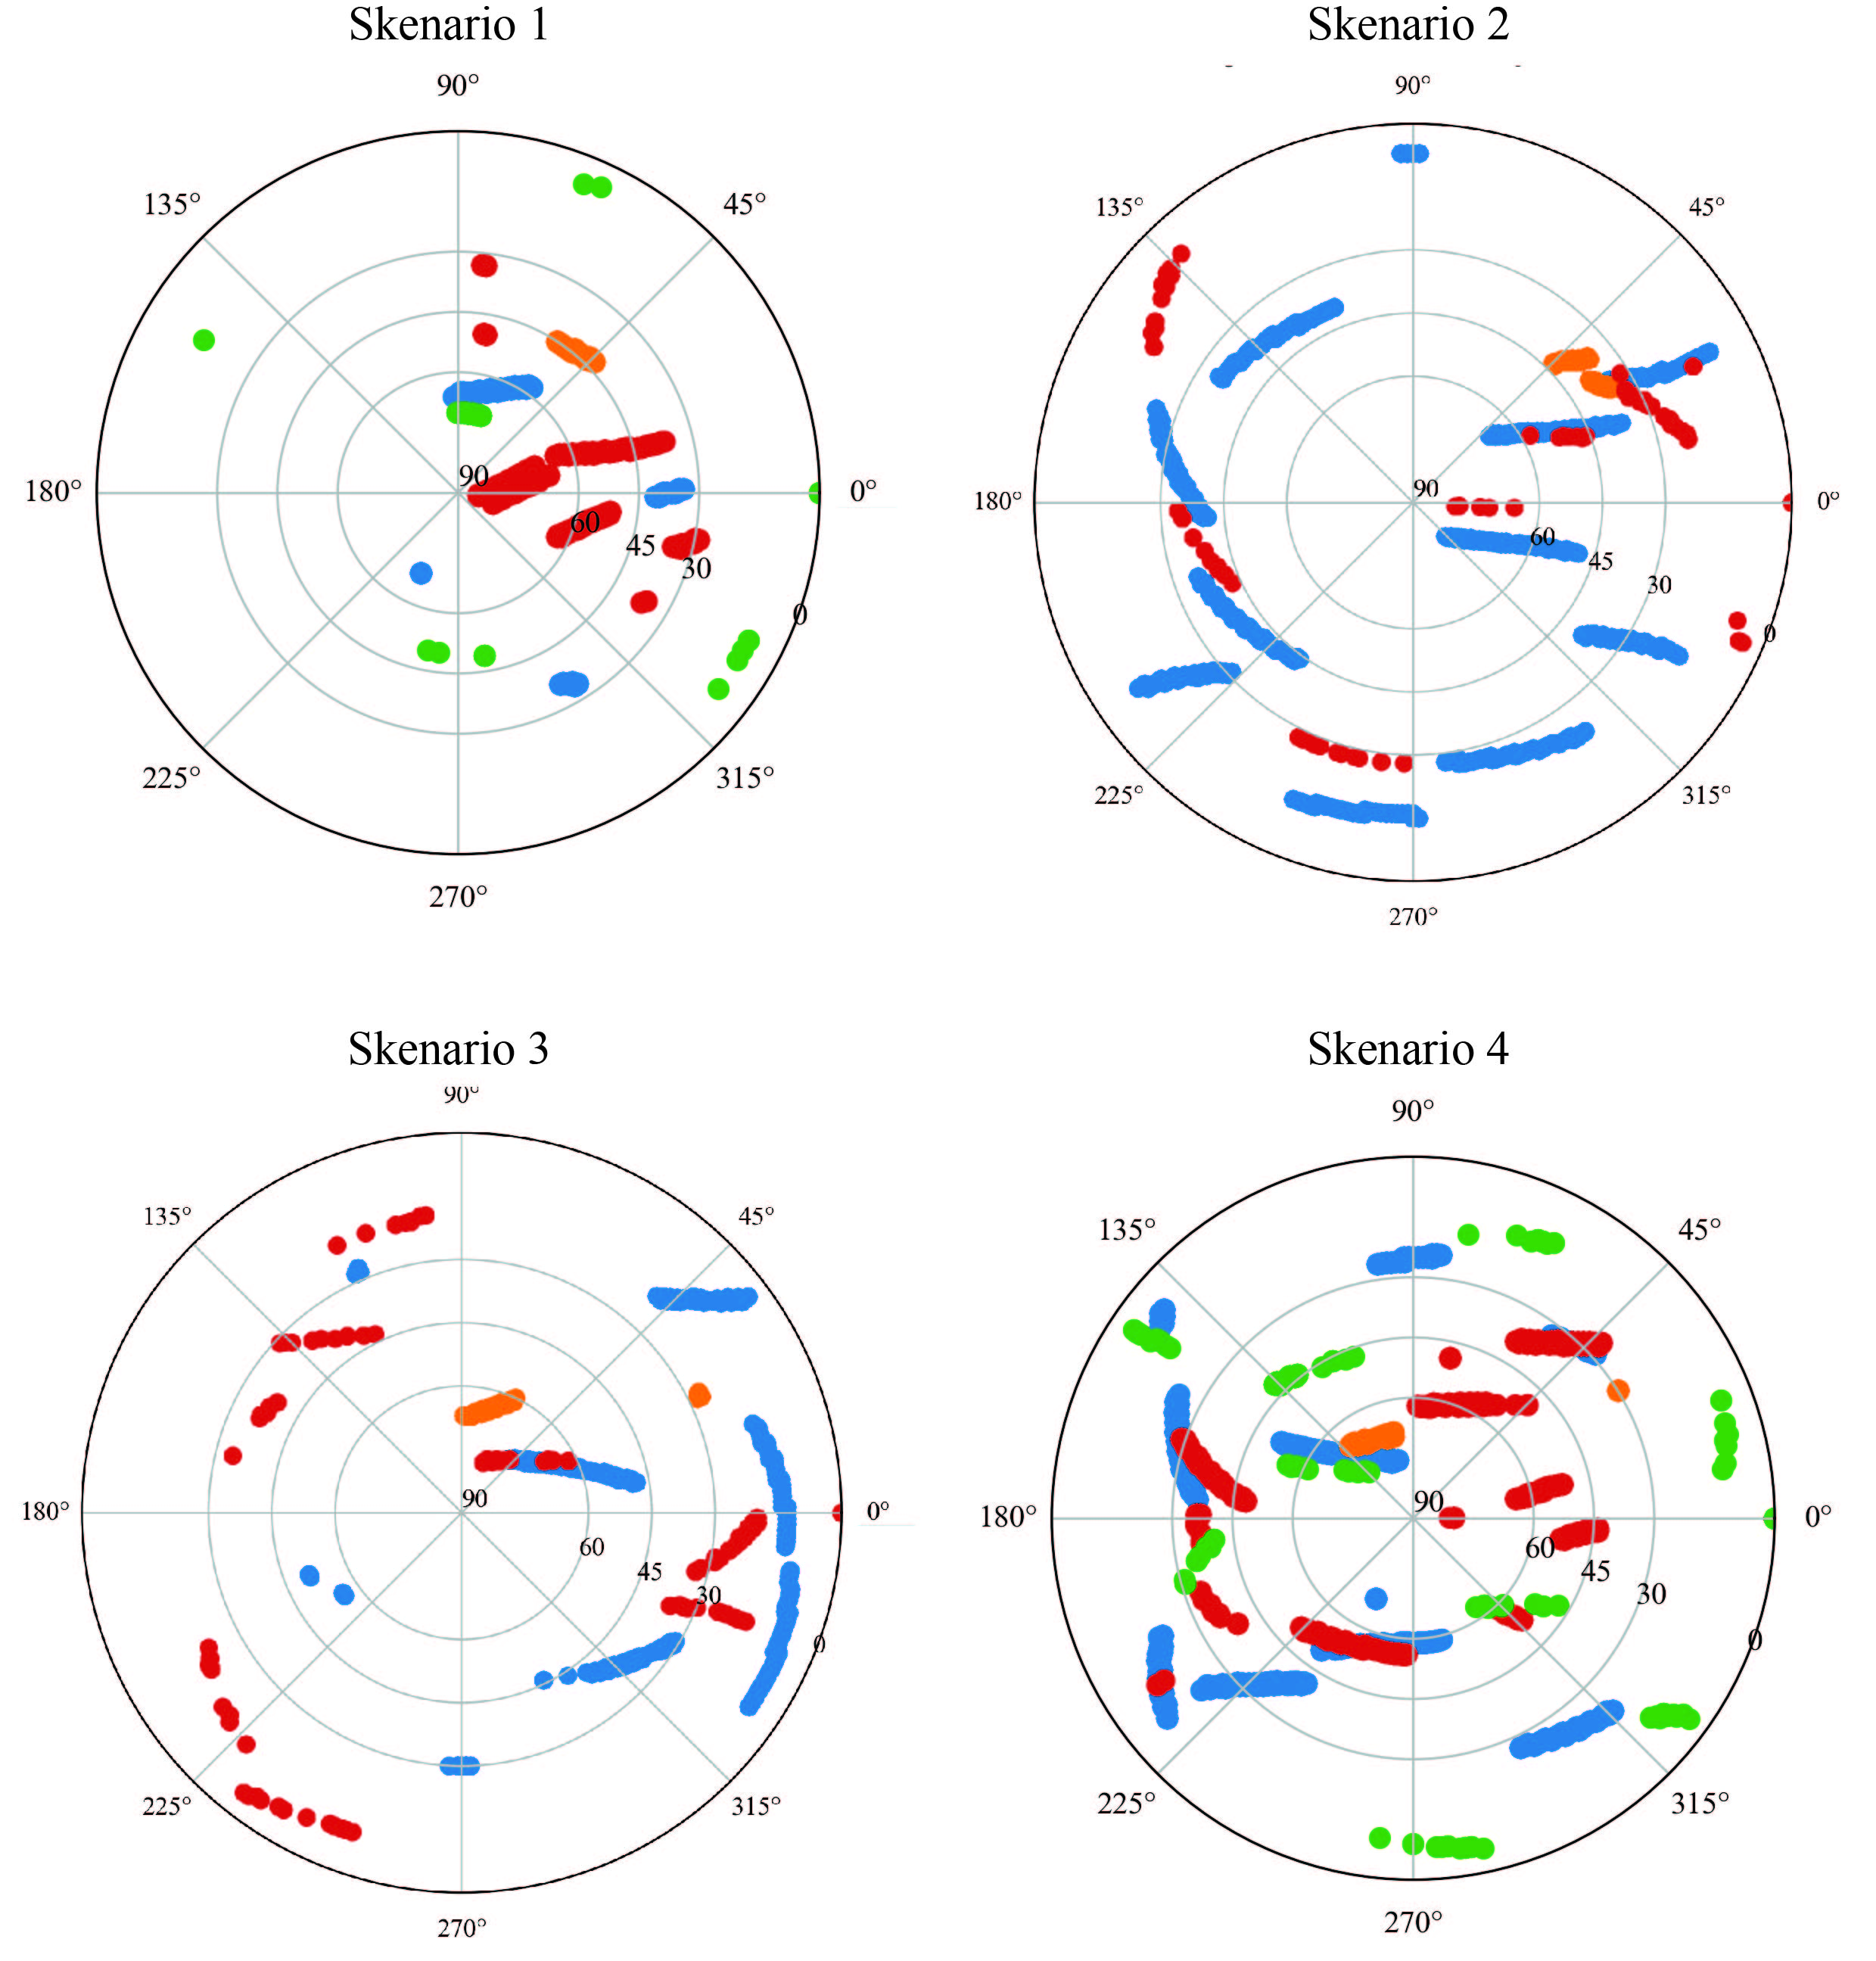
\includegraphics[width=8cm]{skyplot.jpg}
	\caption{\textit{Sky Plot} Hasil \textit{Rapid Static Survey} (Biru: GPS; Merah: BeiDou; Hijau: Galileo; dan Oranye: QZSS)}
	\label{fig: 4-skyplot}
\end{figure}

Tren nilai PDOP cenderung menurun untuk setiap skenario. Nilai PDOP dipengaruhi oleh geometri dari satelit. Sebagai contoh, nilai PDOP pada skenario 1 sangatlah tinggi dan persebaran satelitnya hanya mengisi $\frac{1}{4}$ bagian lingkaran seperti ditunjukan oleh Gambar \ref{fig: 4-skyplot}. Di sisi lain, \textit{sky plot} pada skenario 4 menunjukan bahwa satelitnya lebih tersebar di langit karena memenuhi seluruh lingkaran. Hal tersebut sejalan dengan nilai PDOP-nya yang menurun.

\subsection{Algoritma Mode Daya Rendah}

\subsection{\textit{Geofencing}}
\subsubsection{\textit{Geofencing} di Wilayah Universitas Gadjah Mada}
\subsubsection{\textit{Geofencing} Halte}

\subsection{Pengujian pada Bus Trans Gadjah Mada}

\section{Kesimpulan}

\bibliography{references}{}
\bibliographystyle{IEEEtran}

\end{document}
